\documentclass[a4paper]{article}

%% Language and font encodings
\usepackage[english]{babel}
\usepackage[utf8x]{inputenc}
\usepackage[T1]{fontenc}

%% Sets page size and margins
\usepackage[a4paper,top=3cm,bottom=2cm,left=3cm,right=3cm,marginparwidth=1.75cm]{geometry}

%% Useful packages
\usepackage{amsmath}
\usepackage{graphicx}
\usepackage[colorinlistoftodos]{todonotes}
\usepackage[colorlinks=true, allcolors=blue]{hyperref}

\title{Actividad 7}
\author{Isaac Neri Gómez Sarmiento}
\date{03 de Abril 2018}

\begin{document}
\maketitle

\section{Introducción}

Esta práctica es una continuación de la Actividad 6, en el cual se analiza un sistema de dos resortes acoplados con dos masas. En esta práctica se abarcan las secciones 3 y 4 del artículo \textit{Coupled spring equations} de Temple H. Fay y Sarah Duncan. 
La sección 3 toma en consideración las fuerzas de restitución no lineales, es decir que no sean proporcionales al desplazamiento. 
La sección 4 no solo considera el amortiguamiento y la fuerza de restitución no lineal, sino también toma en cuenta el forzamiento externo.

\section{Añadiendo no-linealidad}
En este apartado se supone que las fuerzas de restitución son no lineales. Tal es el caso de vibraciones grandes en donde el modelo lineal de la ley de Hook $F=-kx$ no describe de manera fiel el movimiento del sistema acoplado, por lo que se puede considerar, como caso particular, que la fuerza de restauración tiene la forma $F=-kx+\mu x^3$. La ecuación diferencial ahora tiene la siguiente forma:

\begin{figure}[ht!]
\centering
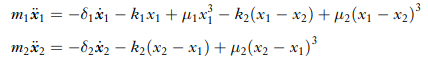
\includegraphics[width=0.7\textwidth]{nonlinearity_eq.PNG}
\end{figure}

Entre más realista se vuelve el modelo, es de esperar que la solución numérica no sea exacta en largos intervalos de tiempo. Lo anterior es debido a errores de redondeo, de truncamiento, de propagación o incluso del algoritmo utilizado. 


\subsection{Ejemplo 3.1}
Asuma $m1=m2=1$. Describa el movimiento para las constantes de resorte $k_1=0.4$ y $k_2=1.808$, coeficientes de amortiguación b1=0 y b2=0, coeficientes no lineales $\mu_1=-1/6$ y $\mu_2=-1/10$, con condiciones iniciales:

\begin{figure}[ht!]
\centering
\includegraphics[width=0.5\textwidth]{initialconditions3_1.PNG}
\end{figure}

El código que se utilizó es muy similar al de la actividad 6, con la diferencia que se agregaron los parámetros $\mu_1$ y $\mu_2$.

\begin{verbatim}
def vectorfield(w, t, p):
    x1, y1, x2, y2 = w
    m1, m2, k1, k2, L1, L2, b1, b2, mu1, mu2 = p
    # Create f = (x1',y1',x2',y2'):
    f = [y1,
         (-b1 * y1 - k1 * (x1) + k2 * (x2 - x1)+ mu1*((x1)**3)+ mu2*((x1-x2)**3)) / m1,
         y2,
         (-b2 * y2 - k2 * (x2 - x1)+ mu2*((x2-x1)**3)) / m2]
    return f

# Use ODEINT to solve the differential equations defined by the vector field
from scipy.integrate import odeint
import numpy as np

# Parameter values
# Masses:
m1 = 1.0
m2 = 1.0
# Spring constants
k1 = 0.4
k2 = 1.808
# Natural lengths
L1 = 0.0
L2 = 0.0
# Friction coefficients
b1 = 0.0
b2 = 0.0

#Non-linear coefficients
mu1=-1.0/6.0
mu2=-1.0/10.0

# Initial conditions
# x1 and x2 are the initial displacements; y1 and y2 are the initial velocities
x1 = 1.0
y1 = 0.0
x2 = -1.0/2.0
y2 = 0.0

# ODE solver parameters
abserr = 1.0e-8
relerr = 1.0e-6
stoptime = 50
numpoints = 500

# Create the time samples for the output of the ODE solver.
# I use a large number of points, only because I want to make
# a plot of the solution that looks nice.
t = [stoptime * float(i) / (numpoints - 1) for i in range(numpoints)]

# Pack up the parameters and initial conditions:
p = [m1, m2, k1, k2, L1, L2, b1, b2, mu1, mu2]
w0 = [x1, y1, x2, y2]

# Call the ODE solver.
wsol = odeint(vectorfield, w0, t, args=(p,),
              atol=abserr, rtol=relerr)

with open('nonlinearsprings3.1.dat', 'w') as f: # Print & save the solution. 
    for t1, w1 in zip(t, wsol): print(t1, w1[0], w1[1], w1[2], w1[3], file=f)
    

\end{verbatim}

\newpage
Las gráficas resultantes son:
\begin{figure}[ht!]
\centering
\includegraphics[width=60mm]{nonlinearsprings3_1_1.png}
\includegraphics[width=65mm]{nonlinearsprings3_1_2.png}
\end{figure}

\begin{figure}[ht!]
\centering
\includegraphics[width=60mm]{nonlinearsprings3_1_3.png}
\includegraphics[width=60mm]{nonlinearsprings3_1_4.png}
\includegraphics[width=60mm]{nonlinearsprings3_1_5.png}
\includegraphics[width=60mm]{nonlinearsprings3_1_6.png}
\end{figure}

\subsection{Ejemplo 3.2}

Asuma $m1=m2=1$. Describa el movimiento para las constantes de resorte $k_1=0.4$ y $k_2=1.808$, coeficientes de amortiguación b1=0 y b2=0, coeficientes no lineales $\mu_1=-1/6$ y $\mu_2=-1/10$, con condiciones iniciales:

\begin{figure}[ht!]
\centering
\includegraphics[width=0.6 \linewidth]{initialconditions3_2_.PNG}
\end{figure}

Las gráficas resultantes son:

\begin{figure}[ht!]
\centering
\includegraphics[width=60mm]{nonlinearsprings3_2_1.png}
\includegraphics[width=60mm]{nonlinearsprings3_2_2.png}
\includegraphics[width=60mm]{nonlinearsprings3_2_3.png}
\end{figure}

\newpage


\subsection{Ejemplo 3.3}

Asuma $m1=m2=1$. Describa el movimiento para las constantes de resorte $k_1=0.4$ y $k_2=1.808$, coeficientes de amortiguación b1=0 y b2=0, coeficientes no lineales $\mu_1=-1/6$ y $\mu_2=-1/10$, con condiciones iniciales:


Para este ejemplo se consideró un tiempo mayor que en los anteriores, para ser específicos, un tiempo de 200 s y 2000 puntos.

\begin{figure}[ht!]
\centering
\includegraphics[width=60mm]{nonlinearsprings3_3_1.png}
\includegraphics[width=65mm]{nonlinearsprings3_3_2.png}
\includegraphics[width=60mm]{nonlinearsprings3_3_3.png}
\end{figure}



\section{Añadiendo forzamiento}
Podemos incluir en nuestro modelo forzamiento externo. Por ejemplo, forzamiento sinusoidal de la forma $Fcos\omega t$, por lo que las ecuaciones diferenciales tendrán la siguiente forma:

\begin{figure}[ht!]
\centering
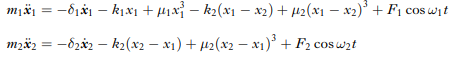
\includegraphics[width=0.7 \linewidth]{forcing_eq.PNG}
\end{figure}

\newpage
En el código se agregan los parámetros $F_1$, $F_2$, $\omega_1$, $\omega_2$.

\begin{verbatim}
import numpy as np
def vectorfield(w, t, p):
    x1, y1, x2, y2 = w
    m1, m2, k1, k2, L1, L2, b1, b2, mu1, mu2, F1, F2, w1, w2 = p

    # Create f = (x1',y1',x2',y2'):
    f = [y1,
         (-b1 * y1 - k1 * (x1) + k2 * (x2 - x1)+ mu1*((x1)**3)+ mu2*((x1-x2)**3)+ F1*np.cos(w1*t)) / m1,
         y2,
         (-b2 * y2 - k2 * (x2 - x1)+ mu2*((x2-x1)**3)+F2*np.cos(w2*t)) / m2]
    return f
\end{verbatim}



\subsection{Ejemplo 4.1}
Asuma $m1=m2=1$. Describa el movimiento para las constantes de resorte $k_1=2/5$ y $k_2=1$, coeficientes de amortiguación b1=1/10 y b2=1/5, coeficientes no lineales $\mu_1=1/6$ y $\mu_2=1/10$, con condiciones iniciales:


\begin{figure}[ht!]
\centering
\includegraphics[width=0.5 \linewidth]{initialconditions4_1.PNG}
\end{figure}


Las gráficas resultantes son las siguientes:

\begin{figure}[ht!]
\centering
\includegraphics[width=60mm]{nonlinearsprings4_1_1.png}
\includegraphics[width=60mm]{nonlinearsprings4_1_2.png}
\includegraphics[width=60mm]{nonlinearsprings4_1_3.png}
\includegraphics[width=60mm]{nonlinearsprings4_1_4.png}

\end{figure}
\newpage
\begin{figure}[ht!]
\centering
\includegraphics[width=60mm]{nonlinearsprings4_1_5.png}
\includegraphics[width=60mm]{nonlinearsprings4_1_6.png}
\includegraphics[width=60mm]{nonlinearsprings4_1_7.png}
\includegraphics[width=60mm]{nonlinearsprings4_1_8.png}
\end{figure}

Podemos observar en las gráficas phaseplot que estas son menos simétricas que las del ejemplo anterior. 
En particular, para las 2 gráficas limit cycle se utilizó un nuevo conjunto de datos generados el cual fue creado con 10000 puntos y un tiempo de 10000 s debido a que este tipo de gráficas se visualiza cuando el tiempo tiende a infinito.

\section{Conclusión}

En esta actividad se tomaron en cuenta dos nuevos parámetros en el análisis del movimiento de un sistema de resortes acoplados. El primero consistia en agregar no linealidad en la fuerza de restauración descrita por la ley de Hook. No se trata más la fuerza de restauración como proporcional al desplazamiento, sino se agrega un término cúbico. 

En el segundo caso se añade un forzamiento externo a la ecuación diferencial. Un ejemplo de ello puede ser que el sistema de resortes no se estire y se libere para que oscile por sí solo y pare debido al amortiguamiento, sino que hay una fuerza externa que hace que el sistema de resortes continue oscilando. 

Al considerar estos parámetros, el análisis se volvió más realista y si se considera un mayor intervalo de tiempo, implica un afectación en la exactitud, ya sea por el algoritmo utilizado o por los errores de redondeo y truncamiento. 

En algunos casos, las gráficas ya dejaban de tener un comportamiento "suave" y simétrico, sino que tenían una apariencia caótica. 

\section{Apéndice}
\begin{enumerate}
\item \textbf{¿Qué más te llama la atención de la actividad completa? ¿Que se te hizo menos interesante?}


La cantidad de parámetros que se pueden añadir a una ecuación diferencial para describir un fenómeno físico lo más aproximado a la realidad.
Por la parte visual me llama la atención las formas interesantes que adquieren las gráficas al considerar más parámetros.


\item \textbf{¿De un sistema de masas acopladas como se trabaja en esta actividad, hubieras pensado que abre toda una nueva área de fenómenos no lineales?}

Anteriormente ya había tratado con resortes y considerado parámetros como el amortiguamiento en la clase de Mecánica II. Sin embargo, no había visto una situación en donde se buscara una nueva expresión no lineal para la ley de Hook. Respondiendo específicamente a la pregunta, si lo habría pensado. 

\item \textbf{¿Qué propondrías para mejorar esta actividad? ¿Te ha parecido interesante este reto?}

Tal y como respondí en el apéndice de la actividad 6, lo que pienso es que habría sido mejor que hubiera consistido en un solo problema, en el cual por equipos hubieramos obtenido experimentalmente las condiciones iniciales, las masas, las constantes de los resortes y los coeficientes de amortiguamiento. De esta manera, proseguiriamos a obtener nosotros las soluciones analíticas a las ecuaciones diferenciales y por último la solución con integración numérica. 

Si me pareció interesante la actividad. Me gustaría que nos ayudara a la interpretación de las gráficas phaseplot y limitcycle.


\item \textbf{¿Quisieras estudiar mas este tipo de fenómenos no lineales?}

Por supuesto que sí. Me gustaría que nos expusiera un problema real al cual usted se haya enfrentado usando herramientas lo aprendido en clase. 


\end{enumerate}

\section{Bibliografía}
\noindent
Temple H. Fay and Sarah D. Graham. Coupled Spring Equations. Recuperado el 12 de Marzo 2018 de: \url{http://math.oregonstate.edu/~gibsonn/Teaching/MTH323010S15/Supplements/coupled_spring.pdf}

Sci-py Cookbook. Coupled spring-mass system. Recuperado el 12 de Marzo 2018 de: \url {http://scipy-cookbook.readthedocs.io/items/CoupledSpringMassSystem.html}

\end{document}